\chapter{Результаты на COSY}\label{chpt4:top-level}

\section{Ускоритель COSY}

\begin{figure}[h]
	\centering
	\includegraphics[scale=.5]{images/chapter4/800px-COSY_Ring}
	\caption{Синхротрон COSY.\label{fig:COSY_Ring}}
\end{figure}

Синхротрон COSY~\cite{COSY-Ring} --- это уникальная установка, позволяющая проводить эксперименты с
поляризованными и охлаждёнными адронными пучками. До конца 2014 года на нём проводились эксперименты
ANKE, PAX, WASA-at-COSY.~\cite{FZJ:Experiments} Начиная с 2015 года, COSY использовался в качестве
полигона для разработки ускорительных и детекторных технологий, а также подготовки и проведения
прецезионных экспериментов с поляризованными пучками: TRIC (Time Reversal Invariance at Cosy) и
JEDI (J\"ulich Electric Dipole moment Investigations).

Для инжекции ионов $H^-$ и $D^-$ в COSY  используется циклотрон JULIC (J\"ulich Light Ion Cyclotron), предоставляющий 8 мкА неполяризованных (или 1 мкА поляризованных) ионов $H^-$ с импульсом 45 МэВ/с. При инжекции отрицательные ионы проходят через углеродный стриппер для изменения их заряда на положительный. Экстракция пучка из циклотрона производится с помощью септум-дефлектора.~\cite{JULIC-Injector}

Возможности направляющей магнитной системы синхротрона ограничивают импульс пучка в диапазоне до 3700 МэВ/с. Экстракция из кольца осуществляется с помощью кикера.

На COSY доступны два типа охлаждения пучка: электронное (диапазон энергий электронов в ``старом'' и ``новом'' кулере -- 20-100 кэВ и 20 кэВ - 2 МэВ, соответственно) и стохастическое. 
%
Два электронных кулера, установленые в кольце на прямой секции, обеспечивают электронное охлаждение во всём диапазоне энергий кольца. Система стохастического охлаждения обеспечивает охлаждение пучка при импульсах 1.5-3.7 ГэВ/с.

Поляризация пучка непрерывно отслеживается на поляриметре  EDDA. Также недавно был установлен поляриметр на основе детекторов WASA, а в конце 2019 года будет установлен новый поляриметр на основе LYSO-сцинцилляторов.
Поляризация протонов достигает 75\% вплоть до наивысших значений импульса; векторная и тензорная поляризации дейтронного пучка достигают 60\%.


В настоящий момент на COSY проводятся исследования по изучению поведения поляризованных пучков в накопительном кольце для будущего эксперимента по измерению ЭДМ в электростатическом кольце.~\cite{Lehrach:Precursor2012, Lehrach:IPAC15, COSY:SpinTuneMapping, Eversmann:SpinTuneMeasurement, COSY:SCT:1000sec, Wagner:BBA2018}
В большинстве исследований были использованы параметры, представленные в Таблице~\ref{tbl:COSY-studies}.

\begin{table}[h]\centering
	\caption{Рабочие параметры COSY, использованные в проводимых исследованиях\label{tbl:COSY-studies}}
	\begin{tabular}{lll}
		\toprule
		Параметр & Величина & Размерность \\
		\midrule
		Длина окружности COSY& 183 & м\\
		Импульс дейтрона & 970 & МэВ/с \\
		 $\beta$ / $\gamma$ & 0.459 / 1.126 & \\
		 Аномальный магнитный момент G& -0.143& \\
		 Частота оборота пучка $f_{\mathrm{rev}}$& 752543& Гц\\
		 Длительность измерительного цикла& 100--1500& сек\\
		 Число частиц в пучке & $\approx 10^9$& \\
		 \bottomrule
	\end{tabular}
\end{table}

Выделим следующие разработки.


\section{Высокоточное измерение спин-тюна}
Пучок дейтронов с вертикально-ориентированным вектором поляризации инжектировался в ускоритель. После подготовительной фазы, во время которой он охлаждался и банчировался, поляризация пучка разворачивалась в горизонтальную плоскость, при помощи ВЧ-соленоида, создающего спиновый резонанс.~\cite[p.~7]{COSY:SpinTuneMapping}

Далее, пучок непрерывно экстрагировался на углеродную мишень, и измерялась асимметрия частоты событий на верхней и нижней секциях детектора, пропорциональная горизонтальной поляризации пучка. Благодаря использованию специально разработанной для этого системы сбора данных,~\cite{COSY:DAQ} было возможно точно определить количество оборотов, сделанных пучком к времени наблюдения события на детекторе.

Проблема измерения заключается в невозможности вычислить спин-тюн путём простого фитирования данных поляриметрии, с $\nu_s$ как оцениваемым параметром, поскольку частота прецессии спина происходит с частотой приблизительно 120 кГц, в то время как частота детектирования событий не превосходит 5 кГц, в связи с чем наблюдалось только одно событие за 24 оборота поляризации вокруг вертикальной оси. Для решения проблемы разреженности данных, был применён алгоритм отображения измерений на период одной осцилляции.~\cite{Eversmann:SpinTuneMeasurement}

В результате была получена беспрецедентная точность определения спин-тюна на уровне $10^{-10}$ в измерительном цикле цикле длительностью 100 секунд, что теоретически позволяет определить величину ЭДМ на уровне $10^{-24}$\ecm.

\section{Юстировка квадруполей при помощи пучка}
\newcommand{\Nbpm}{N_{\mathrm{BPM}}}
Для юстировки положения квадруполя (Beam Based Alignment~\cite{Wagner:BBA2018}), варьируют силу поля квадруполя, и наблюдают за реакцией пучка. Если пучок проходит не через центр квадруполя, он отклоняется. Величина отклонения описывается выражением
\[
\Delta x = \frac{\Delta k\cdot x(s_0)\ell}{B\rho}\cdot \frac{1}{1 - k\frac{\ell\beta(s_0)}{2B\rho\tan\pi\nu}}\cdot \frac{\sqrt{\beta(s)\beta(s_0)}}{2\sin\pi\nu}\cos\bkt{\phi(s) - \phi(s_0) - \pi\nu},
\]
где $\Delta x$ изменение орбиты; $s$ координата, в которой измеряется отклонение пучка; $s_0$ точка расположения квадруполя; $\Delta k$ изменение силы квадруполя; $\ell$ длина квадруполя; $\nu$ бетатронный тюн; $\phi$ бетатронная фаза; $x(s_0)$ положение пучка относительно магнитного центра квадруполя.

Поскольку изменение орбиты $\Delta x(s)$ --- линейная функция отклонения пучка от магнитного центра квадруполя, возможно определить оптимальное положение квадруполя, минимизируя функцию
\[
f = \frac{1}{\Nbpm}\sum_{i=1}^{\Nbpm} (x_i(+\Delta k) -x_i(-\Delta k)^2 \propto x^2(s_0).
\]

Впервые, проверка технологии BBA была проведена в ноябре-декабре 2017 года. Методология требует варьирования силы одного квадруполя за раз, иначе наблюдаемый эффект отклонения пучка будет суперпозицией нескольких отклонений. Поскольку квадруполи на COSY питаются группами по четыре, для варьирования силы поля единичного квадруполя были использованы дополнительные обмотки полюсов некоторых квадруполей. В этом случае, поле квадруполя становится суперпозицией двух квадрупольных полей, но это не отражается на работе методики. 

Для варьирования точки входа пучка в квадруполь использовались кикеры, отклоняющие пучок от референсной орбиты.

Повторная отработка методологии была проведена в феврале 2019 года.

По результатам работы, положения квадруполей были определены с точностью 0.2~мм.~\cite[стр.~182]{YellowReport}

Особенно релевантны для данной работы исследования по оптимизации времени когерентности спина; рассмотрим эту процедуру более подробно.
\section{Оптимизация времени когерентности}\label{sec:COSY:SCT-optimization}
\newcommand{\dpop}{\Delta p/p}

Изначальной целью экспериментов по изучению времени когерентности спина (Spin Coherence Time) на COSY было подтверждение возможности секступольных полей противодействовать дисперсии спин-тюнов, ассоциированной с 
эмиттансом и дисперсией импульсов ($\dpop$) частиц пучка.~\cite{COSY:SCT:IPAC15} На настоящий момент, оптимизация SCT является первой фазой любого предварительного эксперимента по поиску ЭДМ на COSY.

Секступольное подавление декогеренции используется совместно с электронным охлаждением пучка, для
уменьшения его фазового объёма, и банчингом, для подавления линейного вклада дисперсии импульсов частиц 
в декогеренцию. Секступоли, располагающиеся в арках, призваны подавлять эффект декогеренции второго порядка.

Для контроля декогеренции используются три семейства секступолей, которые маркированны соответственно: MXG, расположенный в максимуме дисперсионной функции, и контролирующий эффект декогеренции связанный с $\dpop$; MXS, расположенный в максимуме горизонтальной бета-функции $\beta_x$, и контролирующий дисперсию, связанную с горизонтальными бетатронными колебаниями; MXL, в максимуме $\beta_y$, контролирующий дисперсию, возникающую из-за вертикальных бетатронных колебаний.

\begin{figure}[H]\centering
	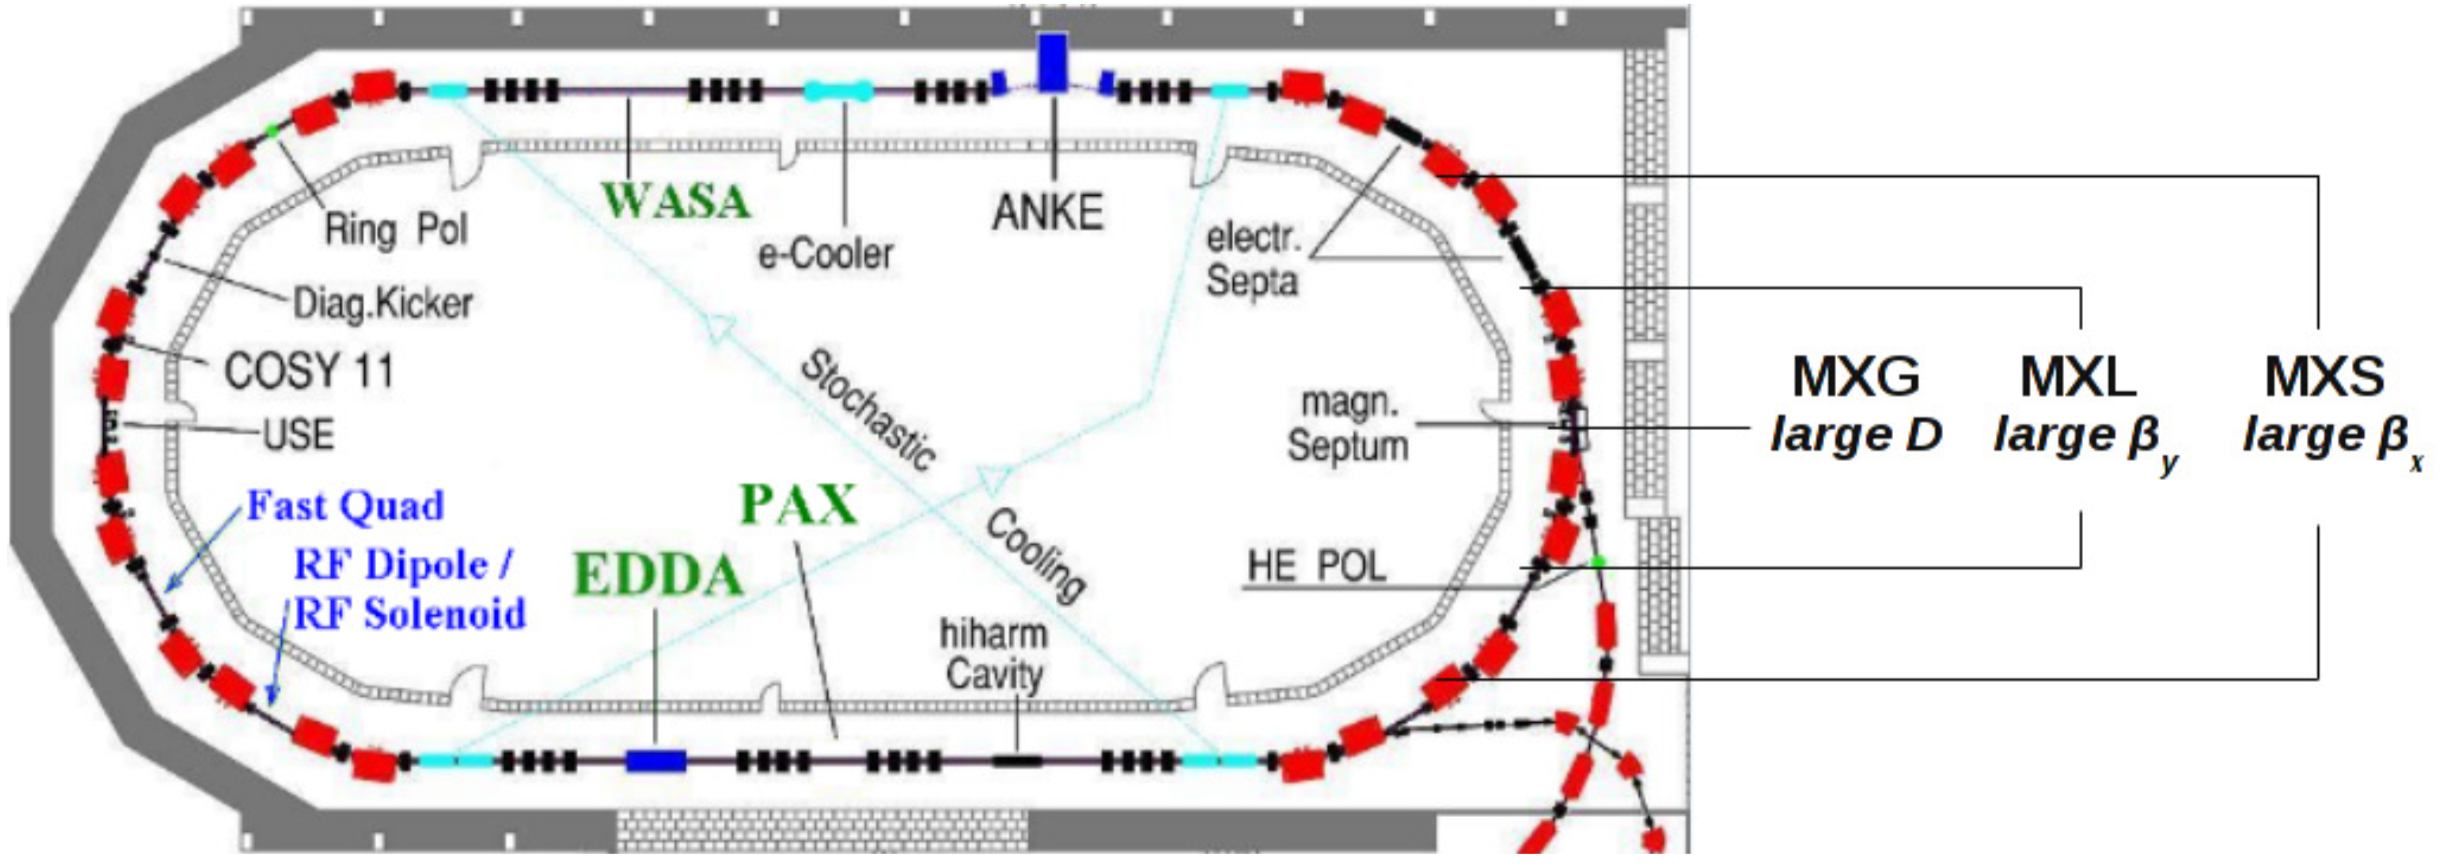
\includegraphics[width=\linewidth]{images/chapter4/COSY-sextupoles}
	\caption{Кольцо COSY с отмеченными положениями секступолей для контроля времени когерентности спина. (Рисунок взят из~\cite{Guidoboni:STORI14})}
\end{figure}

\subsection{Процедура оптимизации}
В этом разделе описана процедура оптимизации SCT, на примере эксперимента 2014 года.~\cite{Guidoboni:STORI14} Первый оптимизационный эксперимент проводился в 2012 году, но тогда варьировалась только напряжённость поля секступоля MXS. В 2014 году впервые проведён полноценный (варьировались градиенты всех трёх секступолей) эксперимент по оптимизации SCT. 

Чтобы отделить эффекты декогеренции, связанные с конечностью эмиттанса пучка, и с вторым порядком дисперсии импульсов частиц $(\dpop)^2$, подготовка пучка к эксперименту проводится по-разному.

Для получения пучка с большим разбросом $(\dpop)^2$, поляризованный дейтронный пучок с импульсом $p=0.97$~ГэВ/с сначала охлаждается в течении 60 секунд для минимизации его эмиттанса. После отключения охлаждения пучок банчируется (гармоническое число $h=1$). Банчирование необходимо для подавления линейных эффектов декогеренции.

В случае изучения декогеренции, связанной с горизонтальным эмиттансом пучка,~\footnote{Декогеренция, связанная с вертикальным эмиттансом не может быть изучена ввиду ограничений по аксептансу.} охлаждение и банчирование проводятся одновременно в течении первых 60 секунд, после чего охлаждение отключается, и на пять секунд включается горизонтальное нагревание. Пучок нагревается подачей белого шума на обкладки конденсатора горизонтального кикера.

В обоих случаях, пучок инжектируется с вертикально-ориентированным вектором поляризации. Поворот поляризации в горизонтальную плоскость производится ВЧ соленоидом, после подготовки пучка, на 80-й секунде.

Мониторинг поляризации пучка производится непрерывно, путём приложения белого шума на вертикальный кикер, для экстракции пучка на 17-мм углеродную мишень. Далее, эластично-рассеянные дейтроны детектируются на поляриметре EDDA. Эластичное рассеяние дейтронов на углеродной мишени чувствительно к направлению спина, и имеет большое сечение взаимодействия. 

Сцинтилляторы поляриметра поделены на четыре группы: верхние, нижние, левые, правые; асимметрия частот событий на левом и правом детекторах пропорциональна вертикальной поляризации, а на верхнем и нижнем --- горизонтальной поляризации. Прецессия поляризации пучка в горизонтальной плоскости происходит с частотой, значительно превышающей частоту выборки поляриметра, поэтому в 2012 году была разработана специальная система сбора данных~\cite{COSY:DAQ}.

По результатам эксперимента~\cite{Guidoboni:STORI14} была доказана возможность получать на COSY SCT 
свыше 1~000~секунд. 

\subsection{Изменение SCT при переходе от внешней к внутренней части пучка}
Ниже представлены результаты оптимизации SCT, полученные в период измерений апрель-май 2019 года. 

На серии рисунков~\ref{fig:April2019:Polarization} представлены измерения асимметрии частоты событий на верхнем и нижнем детекторах (так называемая асимметрия верх-низ), которая пропорциональна горизонтальной компоненте поляризации пучка. На первых двух рисунках можно наблюдать, что на начальном этапе (в промежутке от 100 до 150 секунд) деполяризация происходит со значительной скоростью, но во второй половине цикла скорость деполяризации падает. На Рисунке~\ref{fig:Polariation:recovery-from-halo-to-core} особенно, мы видим, что в промежутке времени приблизительно от 130 до 150 секунд поляризация начинает возрастать, прежде чем снова спадает со значительно меньшей скоростью.
\begin{figure}[H]\centering
	\subbottom[SCT = $20.87 \pm 1.49$ секунд\label{fig:Polariation:recovery-from-halo-to-core}]{%
		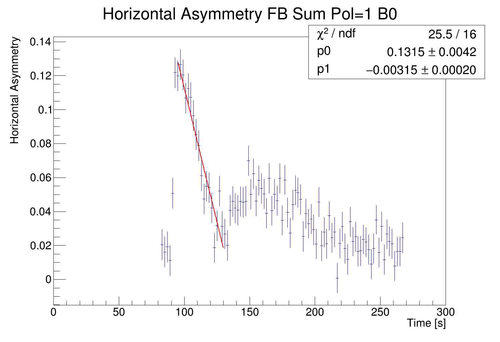
\includegraphics[height=.35\paperheight]{images/chapter4/SCT-April-2019/11th_19-55}}
\end{figure}
\begin{figure}[H]\centering
	\contsubbottom[SCT = $42.3 \pm 2.2$ секунд]{%
		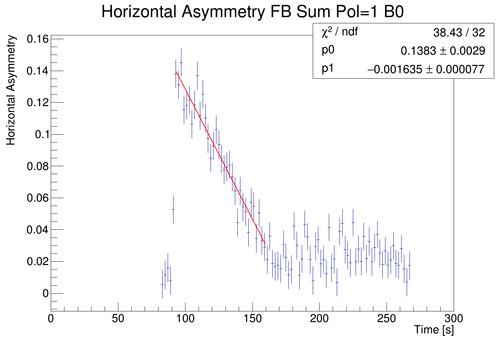
\includegraphics[height=.35\paperheight]{images/chapter4/SCT-April-2019/11th_20-20}}
\end{figure}
\begin{figure}[H]\centering
	\contsubbottom[SCT = $70.6 \pm 4.1$ секунд\label{fig:Polarization:halo-and-core-similar}]{%
		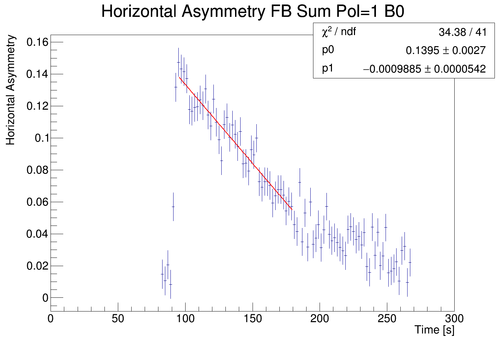
\includegraphics[height=.35\paperheight]{images/chapter4/SCT-April-2019/11th_20-31}}
\end{figure}
\begin{figure}[H]\centering
	\contsubbottom[SCT = $302.0 \pm 27.5$ секунд]{%
		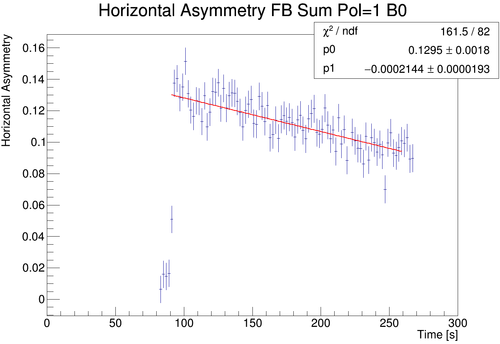
\includegraphics[height=.35\paperheight]{images/chapter4/SCT-April-2019/13th_03-23}}
	\caption{Измерения горизонтальной поляризации во время оптимизации времени когерентности спина при подготовке к эксперименту по поиску аксионов в апреле 2019 года\label{fig:April2019:Polarization}}
\end{figure}

Такое поведение поляризации на данный момент объясняется неоднородностью поляризованности пучка. В первой половине цикла на детектор преимущественно попадают частицы из внешней (halo) части пучка (оболочки); к второй половине цикла начинается выборка частиц из центральной (core) части (ядра). Поскольку ядро плотнее чем оболочка, разброс длин орбит частиц ядра меньше, чем частиц оболочки, а значит меньше и разброс спин тюнов частиц.

\subsection{Зависимость времени когерентности спина от силы секступоля}
На Рисунках~\ref{fig:SCT_scan} представлена зависимость времени когерентности спина от относительной силы поля, соответственно MXL и MXG секступолей, измеренная во время оптимизации в апреле 2019 года. Наблюдается зависимость резонансного типа времени когерентности от значений относительной силы поля секступолей.

\begin{figure}[H]\centering
	\subbottom[Секступоль MXL]{%
		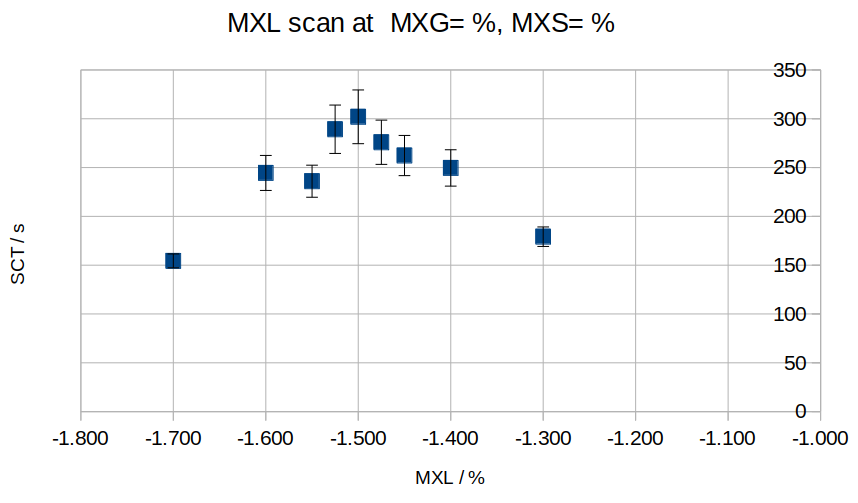
\includegraphics[height=.3\paperheight]{images/chapter4/SCT-April-2019/MXL_scan}}
\end{figure}
\begin{figure}[H]\centering
	\contsubbottom[Секступоль MXG]{%
		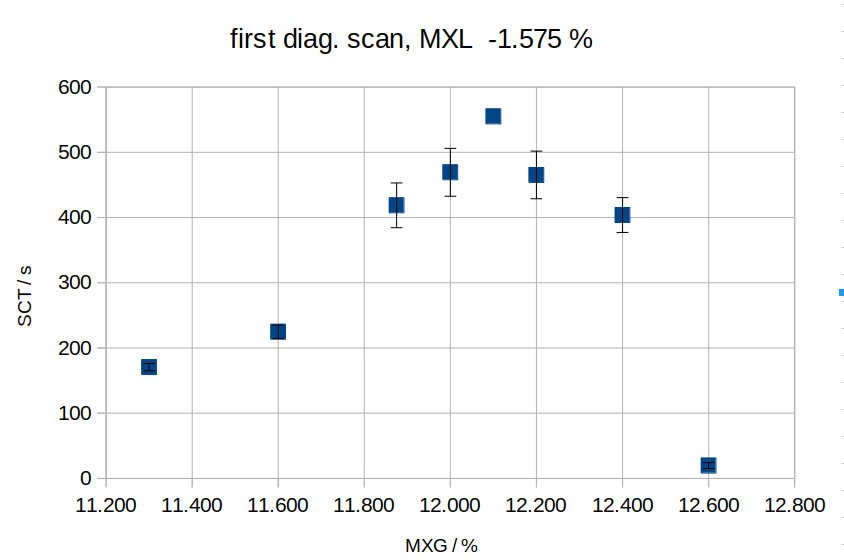
\includegraphics[height=.3\paperheight]{images/chapter4/SCT-April-2019/MXG_scan}
	}
	\caption{Зависимость SCT от градиента секступоля\label{fig:SCT_scan}}
\end{figure}

Мы проверили, соблюдается ли такая же зависимость в рамках нашей численной модели, с учётом того, что измерения на COSY проводятся на энергии, значительно удалённой от спин-резонансной. На Рисунке~\ref{fig:SCT_resonance} изображена зависимость стандартного отклонения спин-тюнов частиц пучка от значения градиента подавляющего декогеренцию секступоля (данные взяты из симуляции, описанной в разделе~\ref{sec:decoh:sim-imperfect}). Зависимость показывает такой же резонансный характер, как и данные эксперимента.

\begin{figure}[H]
	\centering
	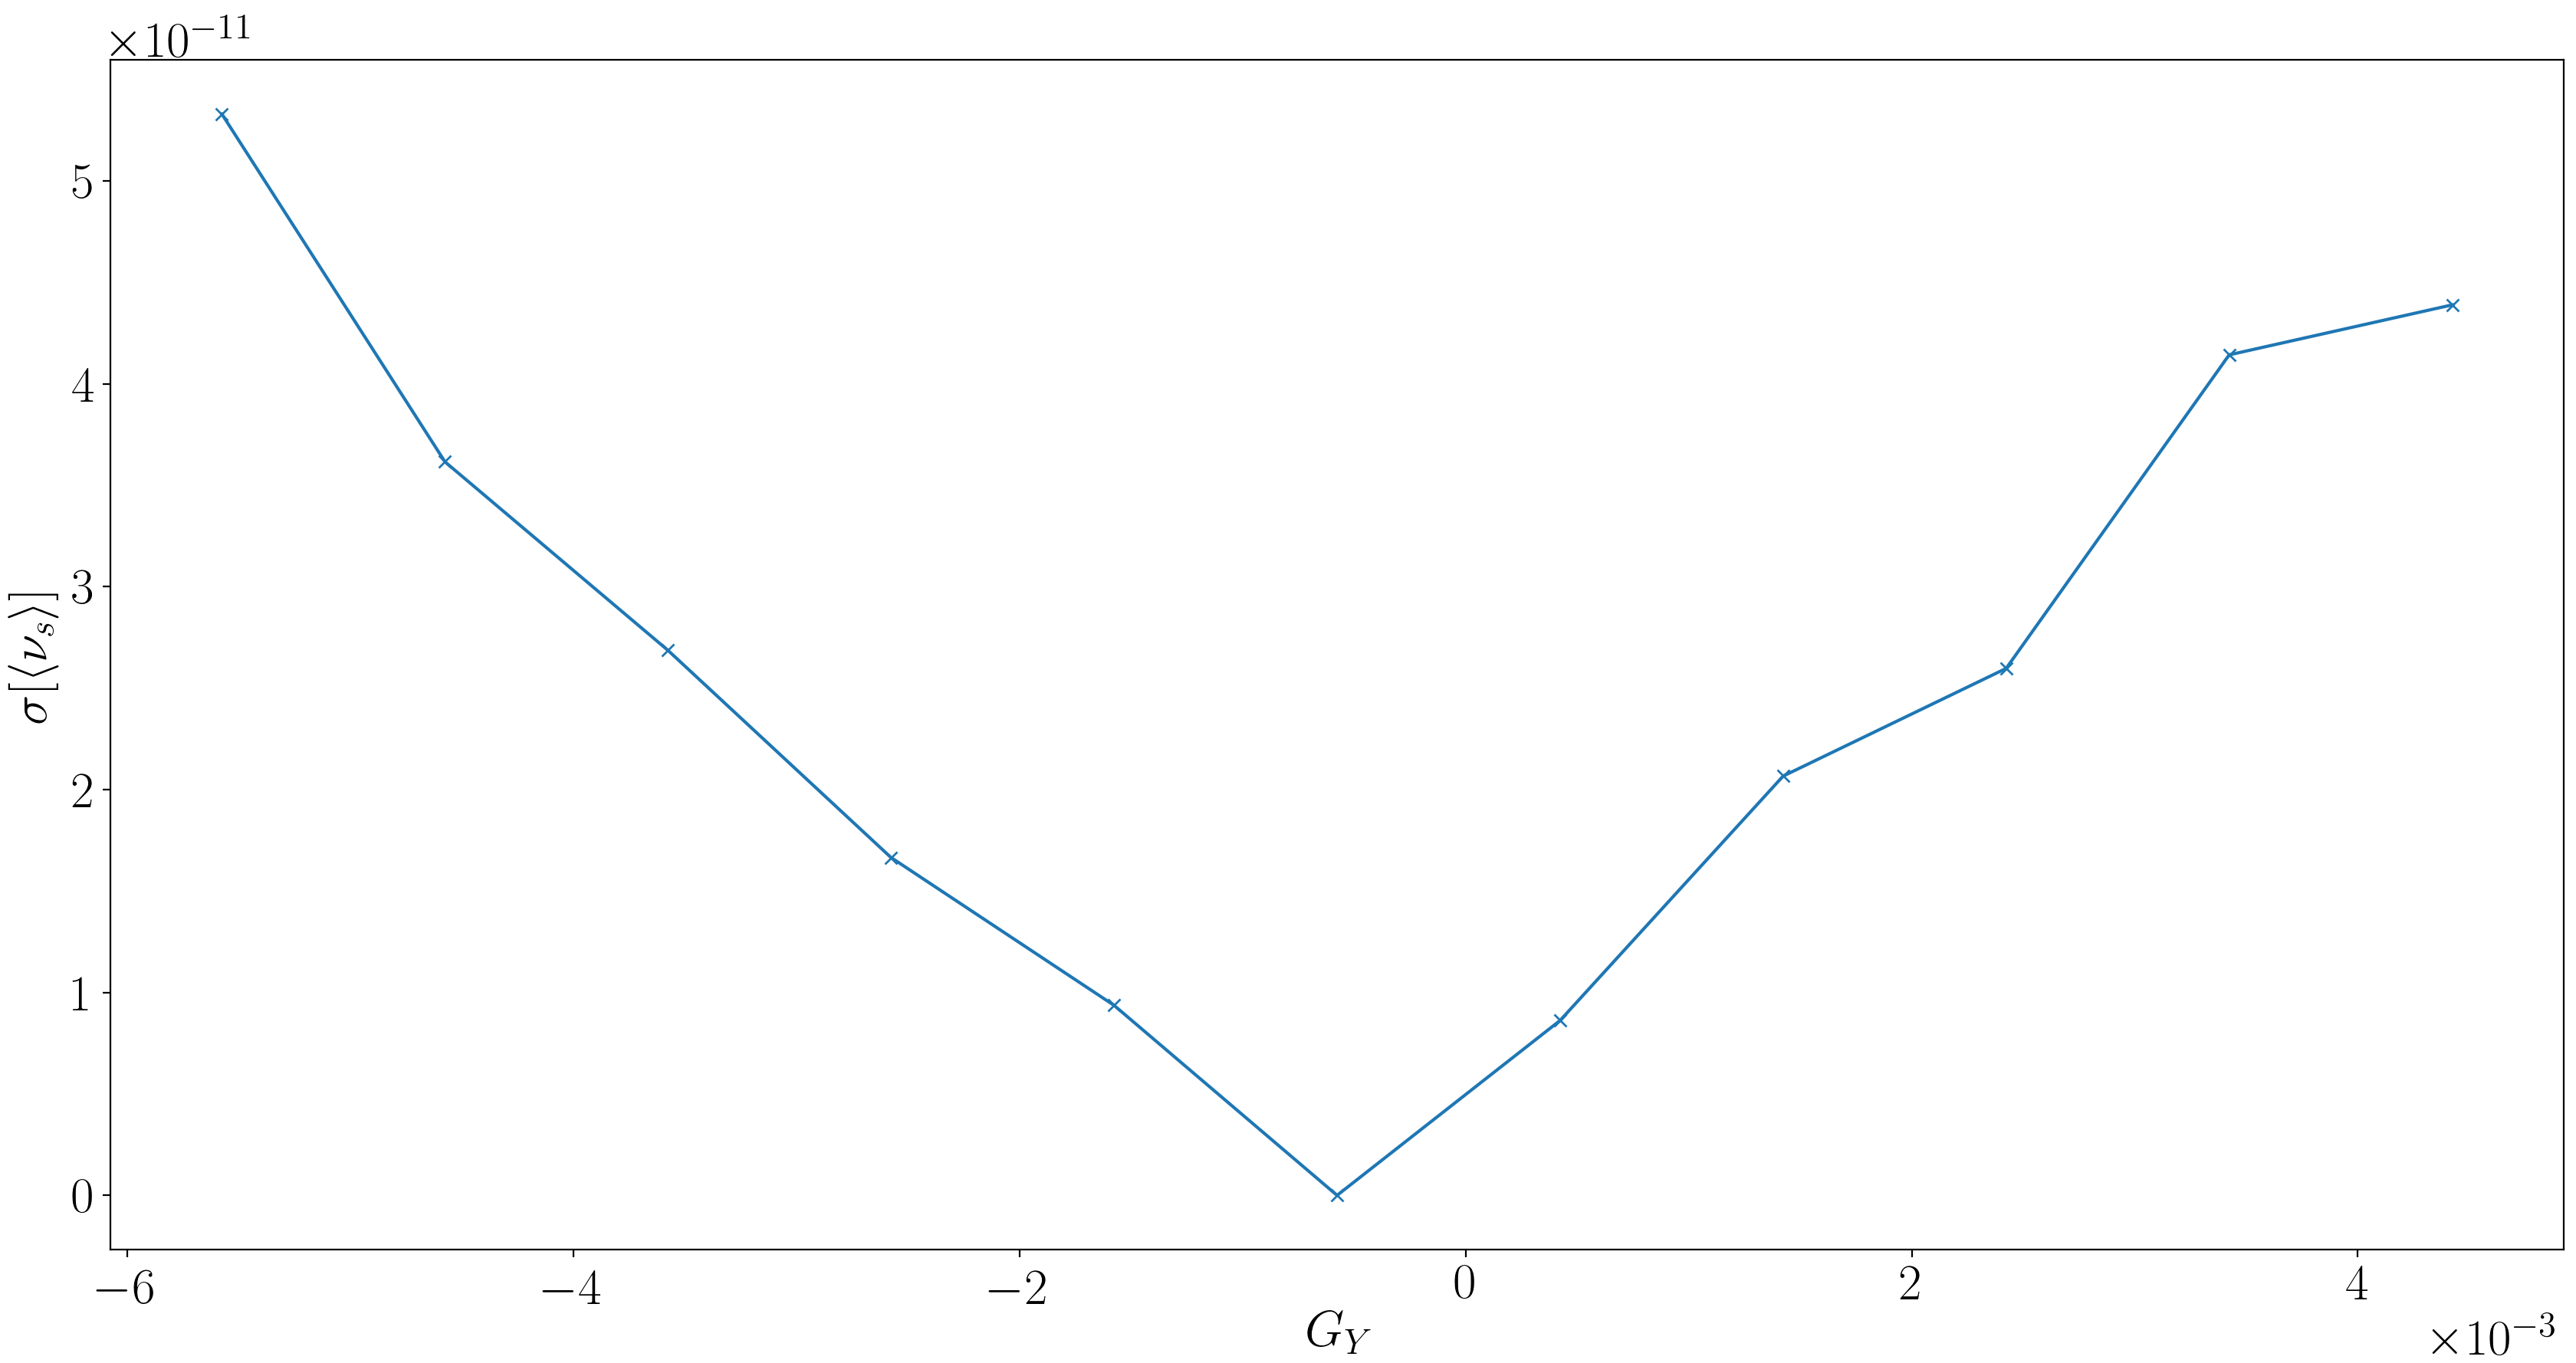
\includegraphics[width=\linewidth]{images/decoh_sim/stune_sd_vs_sext_strength_resonance}
	\caption{Зависимость стандартного отклонения спин-тюнов частиц банча от используемого градиента подавляющего декогеренцию секступоля.\label{fig:SCT_resonance}}
\end{figure}



\clearpage
